\documentclass[tikz,border=10pt]{standalone}
\usepackage{tikz}
\usetikzlibrary{arrows.meta,positioning,calc,backgrounds,fit,shapes.geometric}
\usepackage[scaled=0.92]{helvet}
\renewcommand{\familydefault}{\sfdefault}
\usepackage{amsmath,amssymb}
\definecolor{ink}{HTML}{262624}
\definecolor{mute}{HTML}{8A8984}
\definecolor{line}{HTML}{BDBBB5}
\definecolor{acc}{HTML}{2A78D6}
\definecolor{accbg}{HTML}{F1F6FD}
\tikzset{
  >={Latex[length=2.2mm]},
  every node/.style={text=ink},
  b/.style={draw=line, fill=white, rounded corners=2pt, align=center, inner sep=6pt,
            minimum height=10mm, text width=#1, font=\small},
  b/.default=40mm,
  a/.style={b=#1, draw=acc, fill=accbg},
  a/.default=40mm,
  t/.style={font=\footnotesize, text=mute, align=center},
  e/.style={->, draw=mute, line width=0.6pt},
  ea/.style={->, draw=acc, line width=0.9pt},
  eh/.style={->, draw=acc, line width=0.9pt, dash pattern=on 3pt off 2pt},
}

\begin{document}
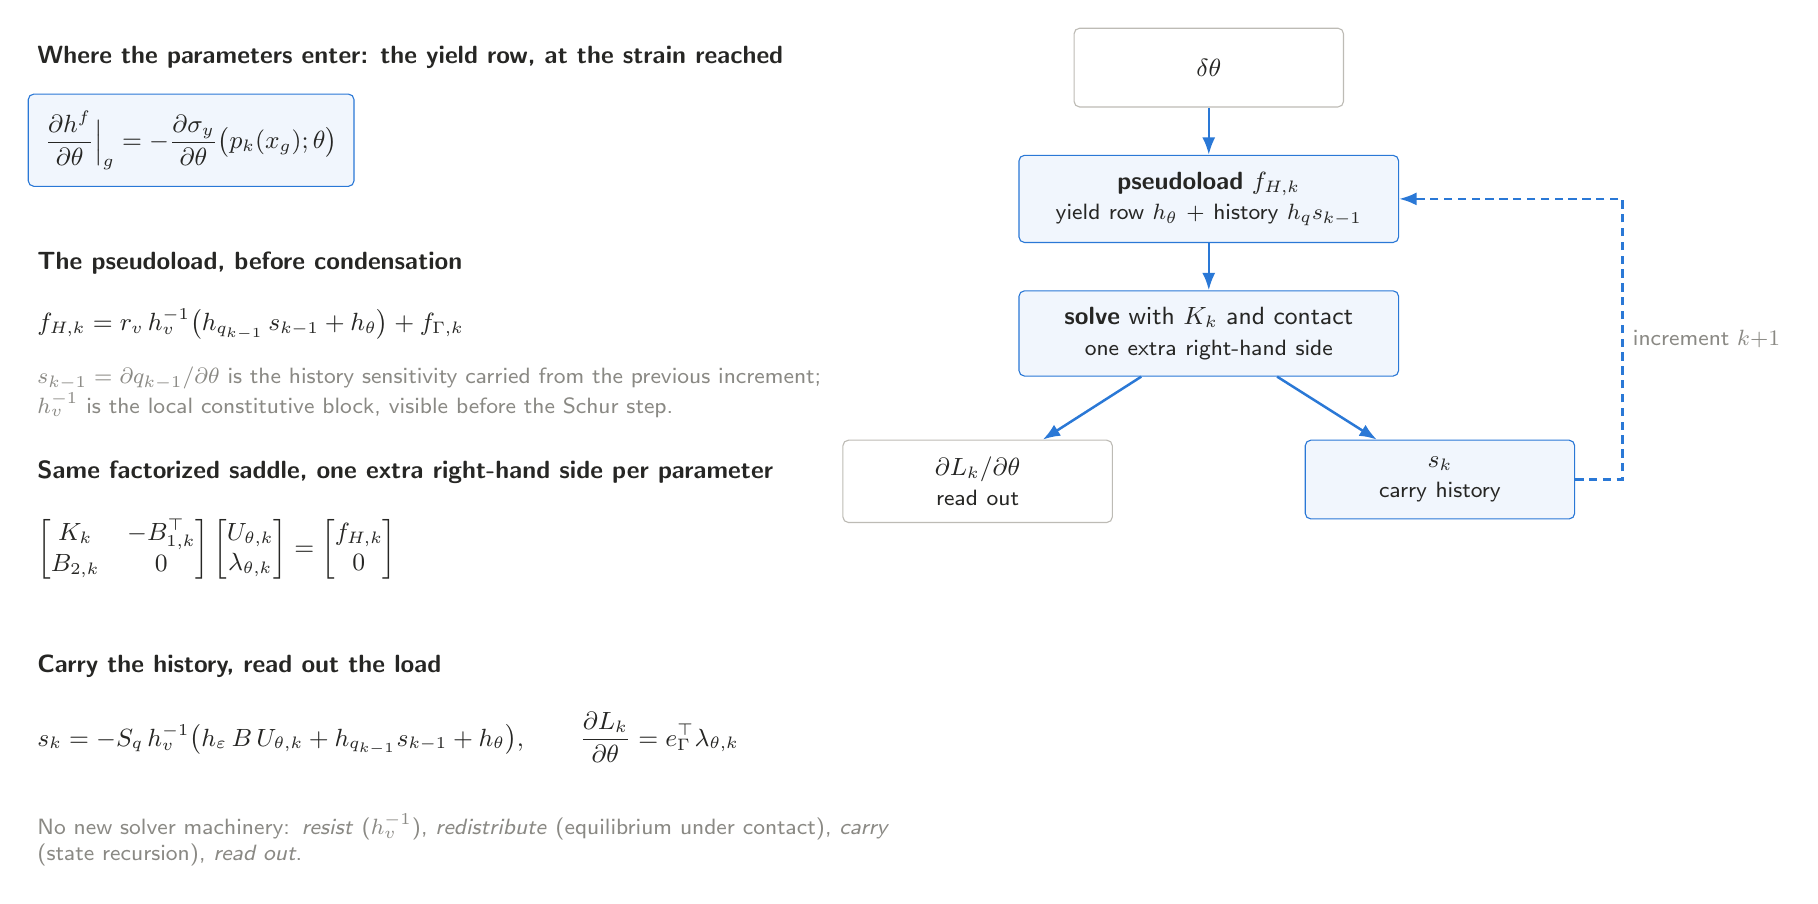
\begin{tikzpicture}[node distance=9mm]
% ---- left: equations ----
\node[anchor=north west, font=\small\bfseries] (h1) at (0,0) {Where the parameters enter: the yield row, at the strain reached};
\node[below=2mm of h1.south west, anchor=north west, font=\small, draw=acc, fill=accbg, rounded corners=2pt, inner sep=6pt] (e1) {%
$\dfrac{\partial h^f}{\partial\theta}\Big|_g = -\dfrac{\partial\sigma_y}{\partial\theta}\big(p_k(x_g);\theta\big)$};
\node[below=7mm of e1.south west, anchor=north west, font=\small\bfseries] (h2) {The pseudoload, before condensation};
\node[below=2mm of h2.south west, anchor=north west, font=\small] (e2) {%
$f_{H,k} = r_v\,h_v^{-1}\big(h_{q_{k-1}}\,s_{k-1} + h_\theta\big) + f_{\Gamma,k}$};
\node[below=1mm of e2.south west, anchor=north west, t, align=left, text width=100mm] {$s_{k-1}=\partial q_{k-1}/\partial\theta$ is the history sensitivity carried from the previous increment; $h_v^{-1}$ is the local constitutive block, visible before the Schur step.};
\node[below=13mm of e2.south west, anchor=north west, font=\small\bfseries] (h3) {Same factorized saddle, one extra right-hand side per parameter};
\node[below=2mm of h3.south west, anchor=north west, font=\small] (e3) {%
$\begin{bmatrix} K_k & -B_{1,k}^{\top}\\ B_{2,k} & 0\end{bmatrix}
\begin{bmatrix}U_{\theta,k}\\ \lambda_{\theta,k}\end{bmatrix}
= \begin{bmatrix} f_{H,k}\\ 0\end{bmatrix}$};
\node[below=7mm of e3.south west, anchor=north west, font=\small\bfseries] (h4) {Carry the history, read out the load};
\node[below=2mm of h4.south west, anchor=north west, font=\small] (e4) {%
$s_k = -S_q\,h_v^{-1}\big(h_\varepsilon\,B\,U_{\theta,k} + h_{q_{k-1}}s_{k-1} + h_\theta\big),\qquad
\dfrac{\partial L_k}{\partial\theta} = e_\Gamma^{\top}\lambda_{\theta,k}$};
\node[below=4mm of e4.south west, anchor=north west, t, align=left, text width=110mm] {No new solver machinery: \emph{resist} ($h_v^{-1}$), \emph{redistribute} (equilibrium under contact), \emph{carry} (state recursion), \emph{read out}.};
% ---- right: flow ----
\begin{scope}[shift={(150mm,-4mm)}, node distance=6mm]
\node[b=30mm] (th) {$\delta\theta$};
\node[a=44mm, below=of th] (pl) {\textbf{pseudoload} $f_{H,k}$\\ {\footnotesize yield row $h_\theta$ + history $h_{q}s_{k-1}$}};
\node[a=44mm, below=of pl] (sv) {\textbf{solve} with $K_k$ and contact\\ {\footnotesize one extra right-hand side}};
\node[b=30mm, below left=8mm and -12mm of sv] (rd) {$\partial L_k/\partial\theta$\\ {\footnotesize read out}};
\node[a=30mm, below right=8mm and -12mm of sv] (cy) {$s_k$\\ {\footnotesize carry history}};
\draw[ea] (th) -- (pl); \draw[ea] (pl) -- (sv); \draw[ea] (sv) -- (rd); \draw[ea] (sv) -- (cy);
\draw[eh] (cy.east) -- ++(6mm,0) |- node[pos=0.25, right, t]{increment $k{+}1$} (pl.east);
\end{scope}
\end{tikzpicture}
\end{document}
